\documentclass{scrartcl}
\usepackage[utf8]{inputenc}
\usepackage{tikz}

\begin{document}
	\title{Evaluating the ArgSearch-prototype}
	\author{Florian Euchner, Nico Weidmann and Nick Heilenkötter}
	\date{Greifswald 2018}
	\maketitle
	
	\section{Task}
	Searching the web for arguments still is a not effectively solved issue. There are some different solution approaches like \texttt{args.me}\footnote{\texttt{args.me} is the prototype implementation of the idea of searching arguments by Wachsmut et al, Bauhaus-Universität Weimar in Weimar, Germany}, but they have not been evaluated well yet. During the 2018 "Sommerakademie" in Greifswald, a scholar workshop of the German National Academic Foundation we attended the work group "Setting the news straight through technology".\\
	Our task was to implement an own search engine based on the \texttt{terrier}\footnote{text}-framework and evaluate diverse retrieval models according to relevance of the results. We did this through a assessor feedback by pooling the results.
	
	\section{The dataset}
	The dataset our search engine uses is the same as the one used by \texttt{args.me} and was provided by its creators.
	To evaluate the search engine, we needed to select some queries which results should be rated by the assessors. Therefore, we analysed the topic coverage of our dataset and  searched the \texttt{/r/ChangeMyView}-dataset to find possible relevant topics. Figure \ref{fig:common_words} shows the amount of selected  words in the titles in both datasets relative to the whole amount of words in the titles. Figure \ref{fig:common_words_arguments} shows the amount of arguments connected to these titles.
		\begin{itemize}
		\item removed arguments longer than 300 and shorter than 5 before indexing
		\begin{itemize}
			\item judging very long arguments (or argumentations) is not effective to the assessors
			\item not possible to argue with less than 5 words
			\item decision based on a look at the distribution (Figure \ref{fig:distr_length})
			\item cause we could not change the dataset \texttt{args.me} uses we were only able to cut the results
		\end{itemize}  
	\end{itemize}
	
	\begin{figure}[hpbt]
	\centering
	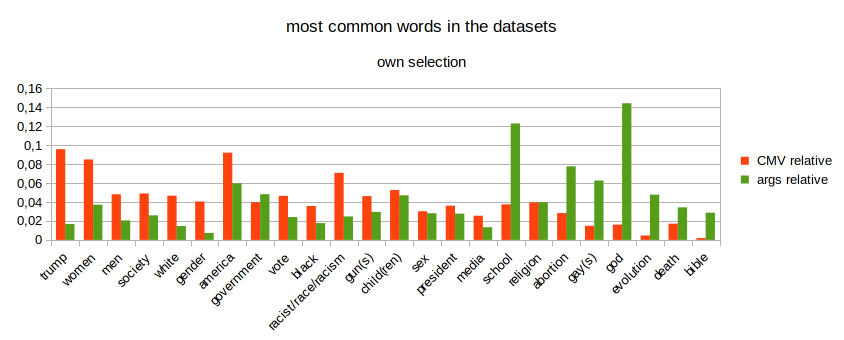
\includegraphics[height=5cm]{img/args_vs_cmv-words.png}
	\caption{most common words in \texttt{args.me}- and \texttt{/r/ChangeMyView}-dataset}
	\label{fig:common_words}
	\end{figure}

	\begin{figure}[hpbt]
	\centering
	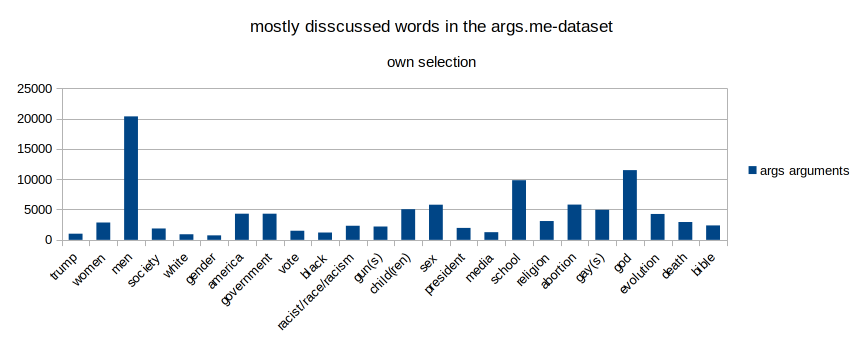
\includegraphics[height=5cm]{img/args_amt_of_arguments.png}
	\caption{mostly discussed topics in \texttt{args.me}-dataset achieved trough counting the number of arguments dealing with topics containing the words in figure \ref{fig:common_words}}
	\label{fig:common_words_arguments}
	\end{figure}
		\begin{figure}[hpbt]
		\centering
		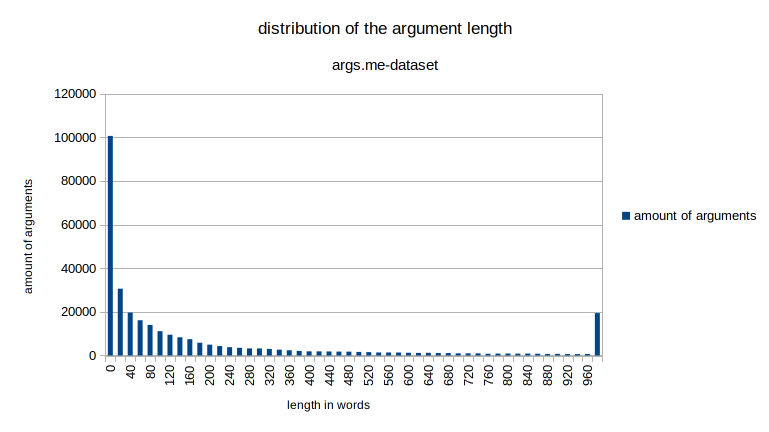
\includegraphics[height=5cm]{img/args_distr_of_length.png}
		\caption{distribution of argument length in \texttt{args.me}-dataset}
		\label{fig:distr_length}
	\end{figure}

	\section{Retrieval models}
	\begin{itemize}
		\item we evaluated 3 terrier retrieval models and \texttt{args.me} by pooling their results
		\begin{itemize}
			\item DPH with MRF Proximity
			\item ...
		\end{itemize}
	\end{itemize}

	\section{Evaluating the retrieval models}
	\begin{itemize}
		\item selection of topics due to both: coverage in dataset and frequently discussed topics in the internet
		\begin{itemize}
			\item chosen topics and querys are accesable in the \texttt{.json}-file
			\item 40 querys with scenarios
			\begin{itemize}
				\item 20 different topics
				\item 1 neutral and 1 biased query + scenario for each topic
			\end{itemize}
		\end{itemize}
		\item we pooled the TOP5 arguments of each platform to reduce the amount of work for the assessors
		\begin{itemize}
			\item average: 12,45 arguments different per query due to the retrieval models finding the same results
			\item amount of different arguments: figure \ref{fig:amt_pooled}
		\end{itemize}
		\item used Google forms as assessor platform
		\item scale of agreement: 1-4
		\item evaluation dimensions based on Wachsmuth et al: ''Computational Argumentation Quality Assessment in Natural Language''
		\item we asked for:
		\begin{itemize}
			\item relevance of the topic to the scenario
			\item rethorical quality
			\item logical cogency
			\item contribution to the discussion
		\end{itemize}
		and gave the assesors the possibility to comment on the argument
		\item we collected the following metadata anonymously:
		\begin{itemize}
			\item age
			\item gender
			\item own opinion about the specific topic
		\end{itemize}
	\end{itemize}
	
	\begin{figure}[hpbt]
		\centering
		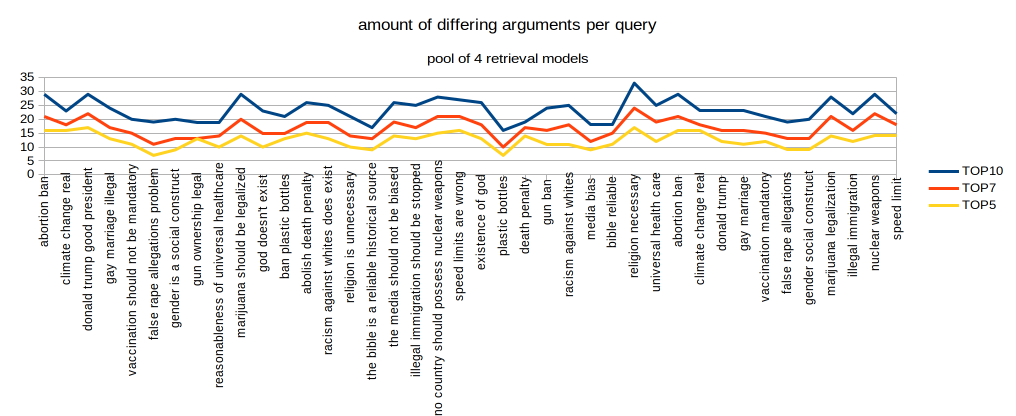
\includegraphics[height=5cm]{img/args_amt_of_pooled_arguments.png}
		\caption{}
		\label{fig:amt_pooled}
	\end{figure}
	
\end{document}